\chapter{Théorie des graphes}
\section{Définitions et concept fondamental (graphe non orienté)}
\subsection{Définitions}
\noindent De façon conceptuelle, un graphe est formé par des sommets (Vertices en anglais) et des arêtes (Edges en anglais) 
qui relient les sommets entre-eux.

\begin{figure}[h]
\centering
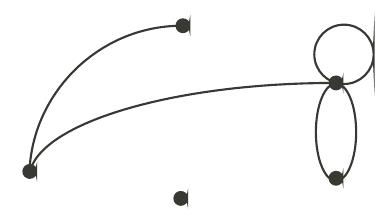
\includegraphics[width=0.5\linewidth]{images/graph}
\caption[Exemple d'un graphe]{Exemple de graphe}
\label{fig:graph}
\end{figure}

\noindent En d'autre terme, un \textbf{graphe} fini noté $G=(V,E)$ est défini par l'ensemble fini $V\ = \{v_{1},\ v_{2},\dots,\ v_{n} \}$ 
dont les éléments sont appelés \textbf{sommets}, 
et par un ensemble fini 
$ E\ = \{ e_{1},\ e_{2},\dots ,\ e_{m} \} $
dont les éléments sont appelés \textbf{arêtes}.

\noindent Une arête $ e $ de l'ensemble $ E $ est définie par une paire non ordonnée de sommets, appelés
les \textbf{extrémités} de $ e $. Si l'arête $ e $ relie les sommets $ u $ et $ v $, on note $ e=\ (u,v) $, on dira que ces sommets sont
\textbf{adjacents}, ou \textbf{incidents} avec $ e $, ou bien que l'arête $ e $ est incidente avec 
les sommets $ u $ et $ v $.\\
Des arêtes sont adjacentes si elle partagent les mêmes extrémités.
On appelle \textbf{ordre} d'un graphe le nombre de sommets n de ce graphe.\\
Les arêtes sont dites \textbf{parallèle} s'ils ont les mêmes extrémités. \\
On appelle \textbf{boucle} l'arête $ e $ de la forme $ (u,u) $. \\
On dit qu'un graphe est un \textbf{graphe simple} s'il ne possède pas des arêtes parallèle et de boucle. \\
Un graphe sans arêtes (c'est-à-dire $E$ est vide )est \textbf{vide}.\\
Un graphe sans sommets (c'est-à-dire $V$ et $E$ sont vides) est un \textbf{graphe nul}.\\
Un graphe avec un seul sommet est dit \textbf{trivial}.\\
Le degré d'un sommet $v$, noté $d(v)$, est le nombre des arêtes qui parent du sommet $v$.
Par convention, une boucle compte deux fois et les arêtes parallèles sont comptées séparément.
Un sommet isolé est un sommet qui a un degré nul.


\begin{figure}[ht]
\centering
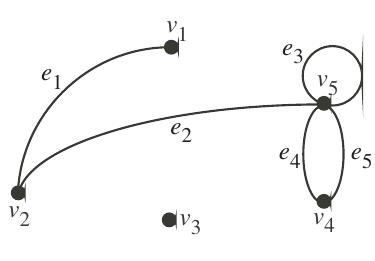
\includegraphics[width=0.5\linewidth]{images/graph1}
\caption[Étiquetage des sommets et des arêtes]{Étiquetage des sommets et des arêtes}
\label{fig:graph1}
\end{figure} 
\paragraph*{}
En prenant l'exemple du Fig. \ref{fig:graph1}:
\begin{itemize}
	\item[\textbullet] $v_{4}$ et $v_{5}$ sont les extrémités de $e_{5}$.
	\item[\textbullet] $e_{4}$ et $e_{5}$ sont parallèle.
	\item[\textbullet] $e_{3}$ est une boucle.
	\item[\textbullet] Ce graphe n'est pas simple.
	\item[\textbullet] $e_{1}$ et $e_{2}$ sont adjacents.
	\item[\textbullet] $v_{1}$ et $v_{2}$ sont adjacentes.
	\item[\textbullet] Le degré du sommet $v_{5}$ est 5.
	\item[\textbullet] Le degré du sommet $v_{4}$ est 2.
	\item[\textbullet] Le degré du sommet $v_{3}$ est 0 donc le sommet est isolé.
\end{itemize}

On note $\delta (G)$ (respectivement $\varDelta (G)$) le degré minimum (respectivement maximum)
des sommets dans le graphe G.
En prenant toujours l'exemple précédent,  $\delta (G) = 0$ et $\varDelta (G) = 5$.
\paragraph*{Remarque.} Dans ce rapport, on considère seulement les graphes finis, c'est-à-dire
$V$ et $E$ sont des ensembles finis.

Comme chaque arêtes ont deux extrémités, on a:

\paragraph*{Théorème 1.1.} Le graphe $G=(V,E)$, où $V = \{v_{1},\dots,v_{n}\}$ et
$E=\{e_{1},\dots,e_{m} \}$, donne
	$$ \sum_{i=1}^{n}d(v_{i})\ =\ 2m  $$
\paragraph*{Corolaire.} Chaque graphe a un nombre pair de sommets d'un degré impair.

\paragraph*{\textit{Preuve.}} Si les sommets $v_{1},\dots,v_{k}$ ont un degré impair et 
les sommets $v_{k+1},\dots,v_{n}$ ont un degré pair, alors (Théorème 1.1.)
$$ d(v_{1}+\dots +v_{k}=2m -\ d(v_{k+1})\ -\ \dots-d(v_{n})$$ 
est pair. D'où, k pair.

En prenant encore l'exemple précédent, la somme des degrés est $ 1+2+0+2+5 = 10 = 2\times 5$.
Il y a deux sommets d'un degré pair qui sont $v_{1}$ et $v_{5}$.

\paragraph*{}
Un graphe est dit \textit{graphe complet} chaque sommet du graphe est relié directement à tous les autres
sommets.
Un graphe complet avec $n$ sommets est noté $K_{n}$. Les quatre premiers graphes complets sont donnés
par Fig.\ref{fig:graph2}. 

\begin{figure}[h]
\centering
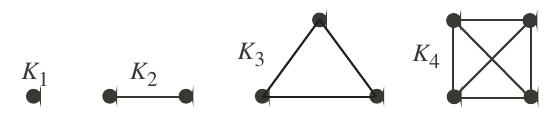
\includegraphics[width=0.5\linewidth]{images/graph2}
\caption[Les quatre premiers graphes complets.]{Les quatre premiers graphes complets.}
\label{fig:graph2}
\end{figure}
\paragraph*{}
\noindent Le graphe $G_{1} = (V_{1},E_{1})$ est un sous-graphe de $G_{2}=(V_{2},E_{2})$ si:
\begin{itemize}
	\item[1.] $V_{1}\subseteq V_{2}$ et
	\item[2.] Chaque arête de $G_{1}$ est aussi une arête de $G_{2}$.
\end{itemize}

\paragraph*{Autres types de graphes}.\\
On appelle \textbf{multigraphes} tous les graphes qui contiennent une boucle, ou
plusieurs arêtes reliant les deux mêmes sommets.

\begin{figure}[h]
\centering
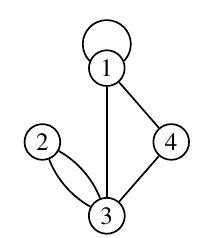
\includegraphics[width=0.2\linewidth]{images/graph3}
\caption[Multigraphe.]{Multigraphe.}
\label{fig:graph3}
\end{figure}

Un graphe est \textbf{connexe} s'il est possible à partir de n'importe quel sommet,
de rejoindre tous les autres en suivant les arêtes. Un graphe non connexe se décompose en composantes
connexes. Sur le graphe ci-dessous, les composantes connexes sont {1, 2, 3, 4} et {5, 6}.
 
\begin{figure}[h]
\centering
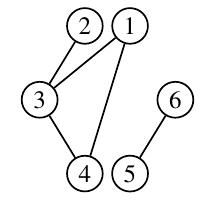
\includegraphics[width=0.2\linewidth]{images/graph4}
\caption[Graphe connexe.]{Graphe connexe.}
\label{fig:graph4}
\end{figure}

Un graphe est \textbf{biparti} si ses sommets peuvent être divisés en deux ensembles X et Y ,
de sorte que toutes les arêtes du graphe relient un sommet dans X à un sommet dans Y
(dans l'exemple ci-dessous, on a X = {1, 3, 5} et Y = {2, 4}, ou vice versa).

\begin{figure}[h]
\centering
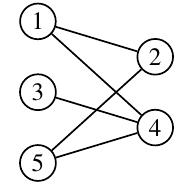
\includegraphics[width=0.2\linewidth]{images/graph5}
\caption[Graphe biparti.]{Graphe biparti.}
\label{fig:graph5}
\end{figure}

\newpage
\subsection{Chaînes et cycles}
Une \textbf{chaîne} dans G, est une suite ayant pour éléments alternativement des sommets et des
arêtes, commençant et se terminant par un sommet, et telle que chaque arête est encadrée
par ses extrémités.
\paragraph*{}
On dira que la chaîne \textbf{relie} le premier sommet de la suite au dernier sommet. En plus, on
dira que la chaîne a pour longueur le nombre d'arêtes de la chaîne.

\begin{figure}[h]
\centering
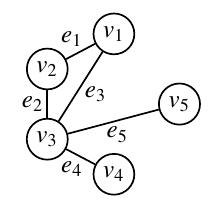
\includegraphics[width=0.2\linewidth]{images/graph6}
\caption[Chaîne.]{Le graphe G contient entre autres les chaînes $ (v_{1} , e_{1} , v_{2} , e_{2} , v_{3} , e_{5} , v_{5} ) $
	et $ (v_{4} , e_{4} , v_{3} , e_{2} , v_{2} , e_{1} , v_{1} ) $.}
\label{fig:graph6}
\end{figure}

\paragraph*{}
On ne change pas une chaîne en inversant l'ordre des éléments dans la suite correspondante.
Ainsi, les chaînes $ (v_{1} , e_{3} , v_{3} , e_{4} , v_{4} ) $ et
 $ (v_{4} , e_{4} , v_{3} , e_{3} , v_{1} )$ sont identiques.
 
\paragraph*{Théorème 1.2.} Un graphe est biparti si et seulement s’il ne contient aucun cycle de longueur impaire.

\paragraph*{Théorème 1.3.} Pour un graphe $ G $ ayant $ m $ arêtes, $ n $ sommets et $ p $ composantes connexes, on définit :
$$ \nu (G) =m-n+p$$
$ \nu (G) $ est appelé le nombre \textbf{cyclomatique}. Prononcer " nu de G ".
On a $ \nu (G) \geq  0$ pour tout graphe $ G $.
De plus, $ \nu (G) = 0 $ si et seulement si $ G $ est sans cycle.


\subsection{Représentations non graphiques d’un graphe}

\subsection{Coupes}

\subsection{Isomorphisme d'un graphe}


\section{Arbres}
\subsection{Arbres et forêts}

\subsection{Circuits et ensembles de coupe}

\section{Arbres couvrants}
\subsection{Définition}

\subsection{Arbres orienté}

\subsection{Graphe orienté acyclique}

\section{Matrices et espace vectoriel d'un graphe}
\subsection{Matrice associé d'un graphe}
\subsection{Matrice d'une coupe}
\subsection{Matrice  d'un circuit}
\subsection{Application: Stationary Linear Networks}
\subsection{Matrices over GF(2) and Vector Spaces of Graphs}

